The operation of modern electricity systems relies heavily on well-structured markets to ensure the balance between generation and consumption. These markets encompass wholesale electricity markets, where energy is traded, and ancillary services markets, which guarantee the system's stability and reliability. The integration of \gls{vRES} has added complexity to these operations, requiring more dynamic approaches to market design and reserve allocation.\par

% \paragraph{Mercado de Serviços de Sistema \label{se:servicos_sistema_mibel}}
% \text{ }  \par
% Por fim, o mercado de serviços de sistema desempenha um papel crítico na manutenção do equilíbrio entre a produção e o consumo de energia elétrica em tempo real. Este mercado é responsável por garantir que a rede elétrica opere de forma segura e estável, ativando reservas e ajustando a produção conforme necessário para responder a variações inesperadas na procura ou na oferta. O mercado de serviços de sistema engloba uma série de mecanismos, incluindo a ativação de reservas de frequência e o despacho de unidades geradoras flexíveis, que são essenciais para a gestão da estabilidade da rede. A participação neste mercado é muitas vezes obrigatória para certos tipos de geradores, especialmente aqueles que possuem a capacidade de resposta rápida, como hidroelétricas e centrais térmicas.\par
% Os mercados de serviços de sistema, português e espanhol, são geridos independentemente, onde o \gls{GGS} é o operador do mercado no respectivo país, sendo a \gls{REN} em Portugal e a \gls{REE} em Espanha.\par
% \bigskip
% \bigskip
% Sumariamente, o \gls{MIBEL} é um mercado complexo e multifacetado que oferece uma ampla gama de formatos de negociação para atender às diversas necessidades dos agentes de mercado. Desde a negociação em tempo real no mercado \textit{spot} até compromissos de longo prazo no mercado de contratação a prazo e acordos personalizados no mercado bilateral, o \gls{MIBEL} proporciona um ambiente robusto para a transação de eletricidade, promovendo a eficiência, a flexibilidade e a segurança do fornecimento de energia na Península Ibérica.\cite{Rassid2017}\par

\subsection{Wholesale Electricity Markets}

Wholesale electricity markets facilitate the trading of electricity between generators, suppliers, and other market participants. These markets are typically divided into three main categories: \gls{DAM}, \gls{IDM}, and real-time balancing markets. In the \gls{DAM}, participants submit bids for energy delivery 12 to 37 hours before real-time operation. The market-clearing process determines the energy schedules and market prices based on supply and demand equilibrium \cite{Algarvio:19b}. While the \gls{DAM} provides a foundation for energy trading, \gls{IDM} allow participants to make adjustments closer to real-time, responding to unforeseen changes in demand or \gls{vRES} generation.\par

Balancing markets, on the other hand, operate in near real-time to address deviations between scheduled and actual energy delivery. \gls{TSO}s procure balancing services to ensure system equilibrium, activating reserves as needed. This process is particularly critical in systems with high \gls{vRES} penetration, where forecasting errors can cause significant imbalances \cite{Algarvio:19a}.\par

\subsection{Ancillary Services and Reserve Requirements}

Ancillary services are essential for maintaining grid stability and ensuring a reliable power supply. They include services such as frequency control, voltage regulation, and operating reserves. Among these, frequency control reserves play a crucial role in balancing supply and demand in real-time. These reserves are divided into three main categories \cite{Algarvio:19a}:

\begin{itemize}
    \item	\gls{FCR}: Activated automatically within seconds to stabilize frequency deviations.
    \item	\gls{aFRR}: Restore frequency to nominal levels and release FCR for subsequent use.
    \item	\gls{mFRR}: Address longer-term imbalances through manual activation.
\end{itemize}

% \begin{figure}[H]
% 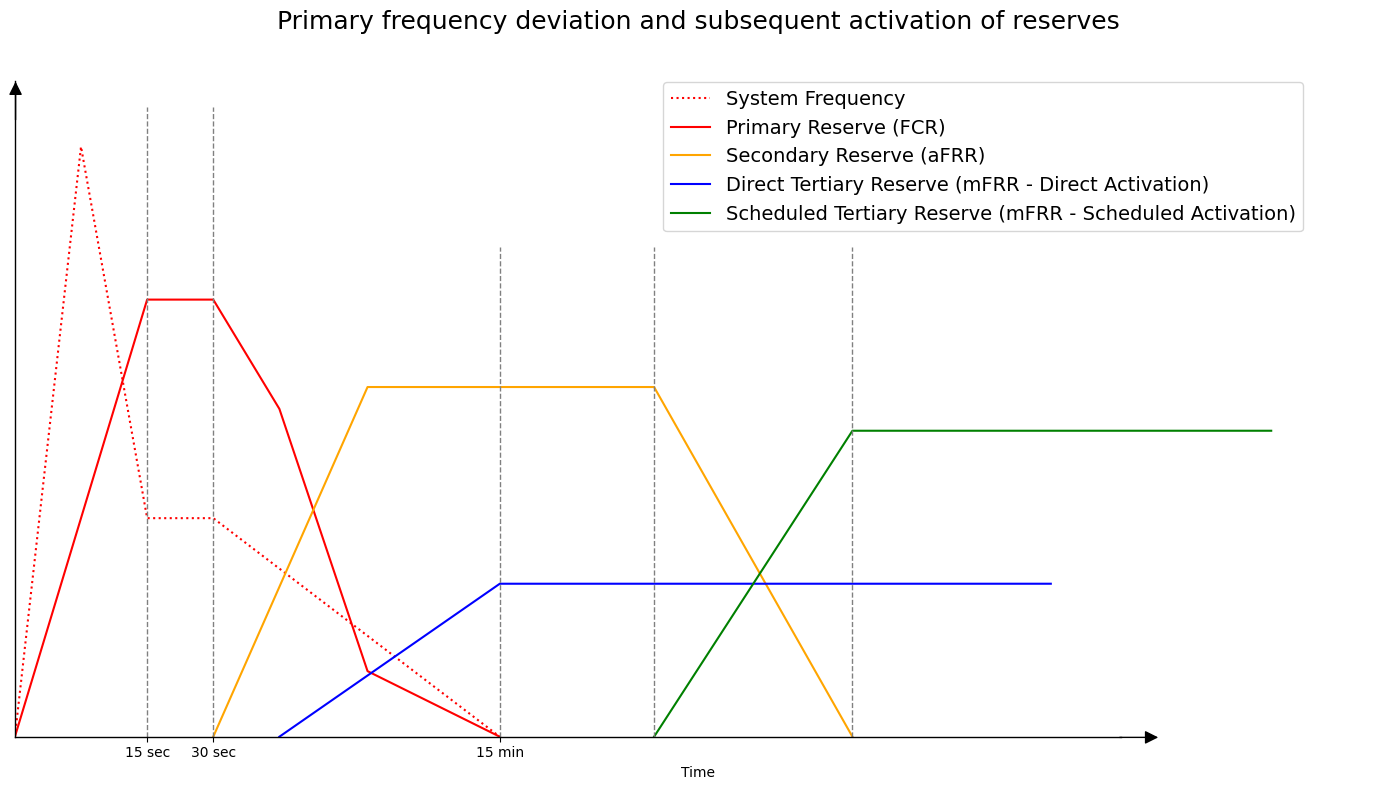
\includegraphics[width=10.5 cm]{plots/actiavtion_example_eng.png}
% \caption{Ancillary Services response scheme. Adapted from \cite{handbook2009policy}}
% \end{figure}   
% \unskip


\begin{figure}[H]
  \centering
  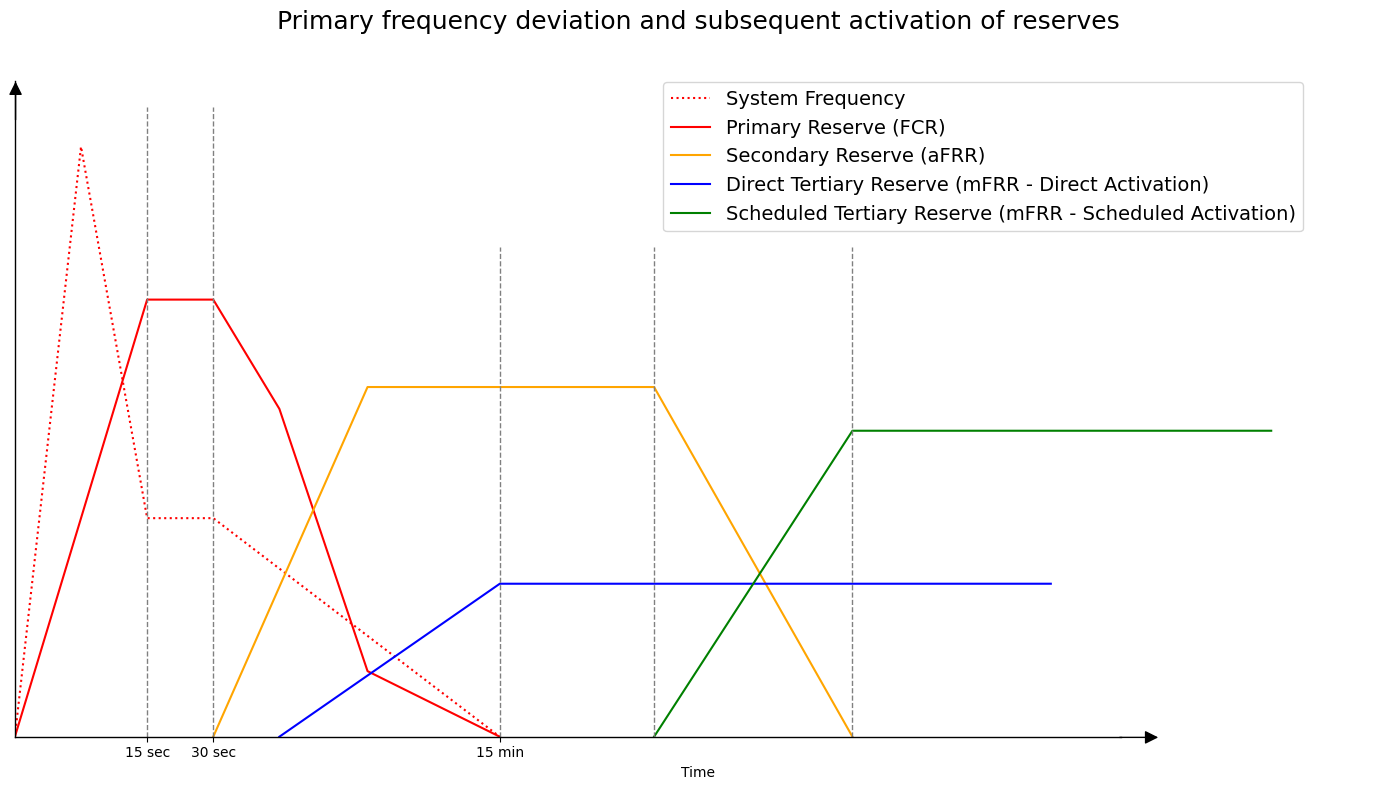
\includegraphics[width=\textwidth]{plots/actiavtion_example_eng.png}
  \caption{Ancillary Services response scheme. Adapted from \cite{handbook2009policy}}
  \label{fig:Ancillary_Services_response_scheme}
\end{figure}
\unskip



\subsection{Iberian Reserve Markets}

\gls{MIBEL} is the iberian example of energy market integration across countries. Acting as a bond between portuguese and spanish electricity markets, \gls{OMIP} and \gls{OMIE}. This joint market consists of bilateral, derivatives, and spot markets.\par
Even though there is a joint market, each country's \gls{TSO}, \gls{REE} for Spain and \gls{REN} for Portugal, manages it's own ancillary services independently. 

\subsubsection{Static Reserve Procurement}
In Europe, the \gls{ENTSO-E} provides guidelines for the procurement and activation of these reserves. Traditionally, \gls{TSO}s acquire reserves symmetrically (equal upward and downward capacities), based on deterministic demand forecasts. However, this approach often leads to inefficiencies in systems with high \gls{vRES} variability.
%
For secundary reserve \gls{ENTSO-E} proposes:
\begin{linenomath}
\begin{equation}\label{eq:BRENTSOE} 
    R = \sqrt{a \times  L_{max} + b^{2}} - b 
\end{equation}
\end{linenomath}
where:

\begin{itemize}
  \item $R$: Secondary Control Reserve.
  \item $a$ and $b$: empiric coefficients, $a$=10MW and $b$=150MW .
  \item $L_{max}$: maximum anticipated consumer load.
\end{itemize}

The Spanish and Portuguese markets provide examples of differing reserve procurement methods. In Portugal, the \gls{TSO} employs a fixed ratio formula for secondary reserve sizing. Creating a symmetrical distribution for upward and downward bands, respectively $\frac{2}{3}$ and $\frac{1}{3}$ of the reserve band.\par
The given formula is based on \gls{ENTSO-E} equation \eqref{eq:BRENTSOE}, adding an hourly ratio $\rho$:

\begin{linenomath}
  \begin{equation}\label{eq:BRREN} 
    R = \rho \times \sqrt{a \times  L_{max} + b^{2}} - b 
  \end{equation}
  \end{linenomath}

The hourly ratio $\rho$ varies between 20\% (1.2) and 60\% (1.6), upscaling the the ENTSO-E suggestion for up regulation.

Conversely, the Spanish market lacks a standardized reserve procurement formula, relying instead on a more flexible procurement mechanism \cite{Frade2019_market}. Where the upward and downward bands distribution is not directly symmetric.
These differences highlight the need for market design improvements to better accommodate the variability of \gls{vRES}.



